\chapter{ABS Filament Production}
\renewcommand{\baselinestretch}{\mystretch}
\label{chap:ABS}
%\setlength{\parindent}{0pt}

\section{Methodology}
The aim of this project is producing printable filament with Lunar and Mars dust simulants. First of all, it is essential to test the printability of the basic material that is ABS pellets (INEOS Styrolution Group GmbH, Germany) and get suitable candidate filament for our 3D printer (Ultimaker 2 GO; Ultimaker B.V., Netherlands). The extruder called Noztek Pro in our experiment is produced by Noztek Company (England, UK), which offers fast extrusion of ABS pellets with tight tolerances. For the good quality of filament, the filament winder (Noztek, England, UK) worked with the extruder as Figure \ref{Fig:extruder and winder} shows.

\begin{figure}[htbp] % make the image in the middle of paragraph
	\centering
	\subfigure[]{
	\begin{minipage}[t]{0.4\textwidth}
			\centering
			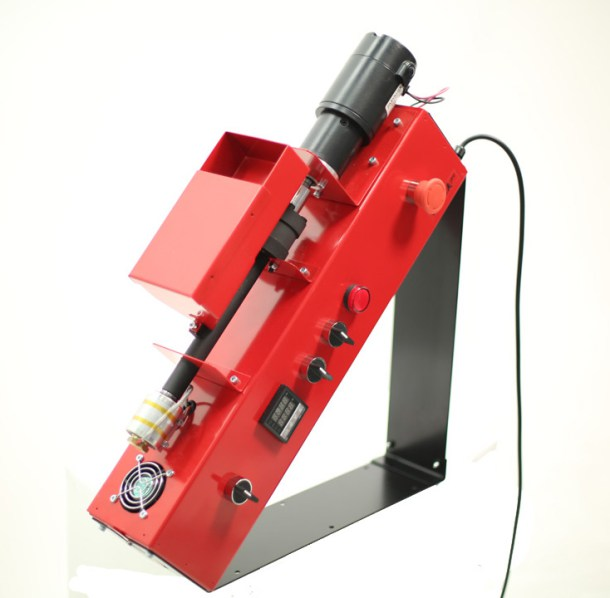
\includegraphics[height=6.1cm]{Figs3//noztek_pro.jpg}
		\end{minipage}
	}
	\subfigure[]{
		\begin{minipage}[t]{0.4\textwidth}
			\centering
			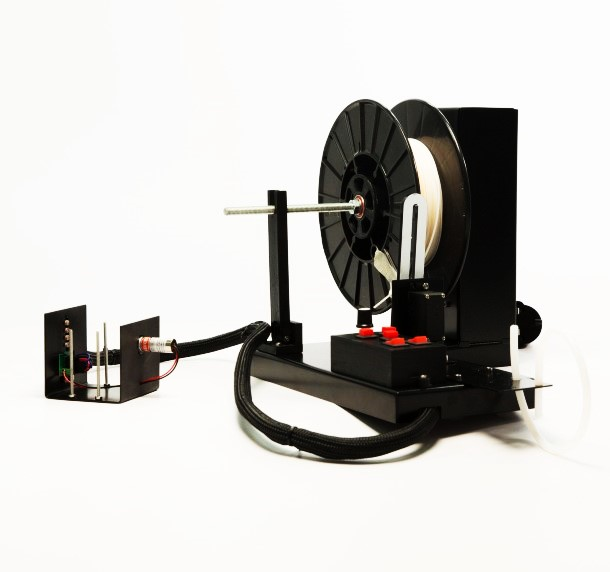
\includegraphics[height=6.1cm]{Figs3//winder1-crop.jpg}
		\end{minipage}
	}
  \caption[The machines for filament manufacuring]{\footnotesize (a) The extruder,(b)the filament winder. Copyright@ Noztek Co. }
  \label{Fig:extruder and winder}
\end{figure}

\subsection{ABS pellets}
As mentioned in Chapter Two, ABS was chosen as the base material due to its compatible property and the reasonable price. The mechanical properties like impact resistance and roughness\cite{swetham2017critical} of ABS also were taken into consideration.
In the view of the ABS pellets in Figure \ref{Fig:ABS pellets}, the colour is white and the size is fairly uniform. It should be noted that the storage of ABS pellets is significant as ABS pellets could absorb moisture from the air in general. As the ABS pellets were purchased in bulk, the solution was to separate the big bulk of pellets into small bags and keep them in a desiccator with desiccants before extrusion. Approximately, each kilogram of ABS pellets could produce 30 meters filament with 3mm diameter. Based on this approximation, 25kg ABS pellets were prepared for the total study.

\begin{figure}[t]
  \centering
  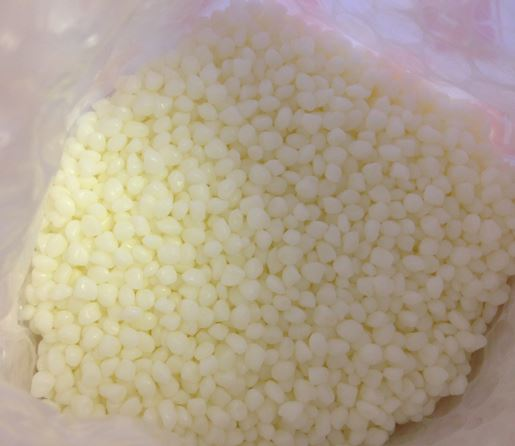
\includegraphics[scale=0.5]{Figs3//ABS_pellets.JPG}
  \caption[ABS pellets]{\footnotesize ABS pellets.}
  \label{Fig:ABS pellets}
\end{figure}

\subsection{Installation of Extruder and Winder}
In the factory, there are five steps for filament production, including extrusion with the extruder, cooling by a water tank, pulling with pull roller, cutting or removal by controlled winder and drying. As there was no oven or other available drying facilities, only the extruder and filament winder with a sensor were facilitated for filament manufacturing in this project. The composition of the extruder is described in Figure \ref{Fig:extruderexp}.\\
\\
In FDM 3D printing, it is necessary to note that the computer controls the printing process by calculating the extruded material's volume, which relies on the extrusion speed, the size of the die in nozzle head and the diameter of the filament. To be specific, the 3D printer controls the filament feeder to push a certain length of filament out of the nozzle by supposing its diameter is consistent. In this way, the unstable filament will cause the volume of extruded plastic changeable since the computer cannot identify the diameter variation. Therefore, the printing is continued with a setting of filament diameter and the printer expects a certain volume of material to come out. This trouble called inconsistent extrusion results from the poor diameter tolerance of filament.\\
\\
In order to avoid this bad printing, the ideal diameter of the filament is 2.85mm for Ultimaker 2 printer. Unfortunately, there are only two sizes of dies we can choose for extrusion nozzle, which are designed for the 1.75mm and 3mm filament production respectively. Consideration of ABS expansion at high temperature, the 1.75mm die was installed.  \\
\\
The reason why we facilitate filament winder is that it could improve the filament tolerances and collect all extruded filament neatly onto the spool. The filament winder was installed on a more robust chassis to offer the smooth and stable winding of 1Kg of the filament. It also connects a sensor and programmable laser module which calculates the extrusion speed of filament by monitoring the height of the filament, in turn changing the speed of the spool motor to give tangle free winding.\\
\\
The guide work of filament winding is similar to a fishing reel leveller. It is related to the spool motor's work record. The guiding part is programmed to rotate about 1 degree after each circle rotation of the spool. In fact, the extrusion product is winded on a standard wound spool which can be used directly to the 3D printer. Since there were not enough available spool for our samples, we re-winded the filament from the installed spool every time we finished extrusion.\\
\\
The entire system could be seen in Figure \ref{Fig:system}. The extruder was located on the desk in order to let filament drop down naturally while the winder was put on a lower place with the sensor in the middle of them. The vertical drop and horizontal distance between each machine would be adjusted during the experiment.

\begin{figure}[htbp]
  \centering
  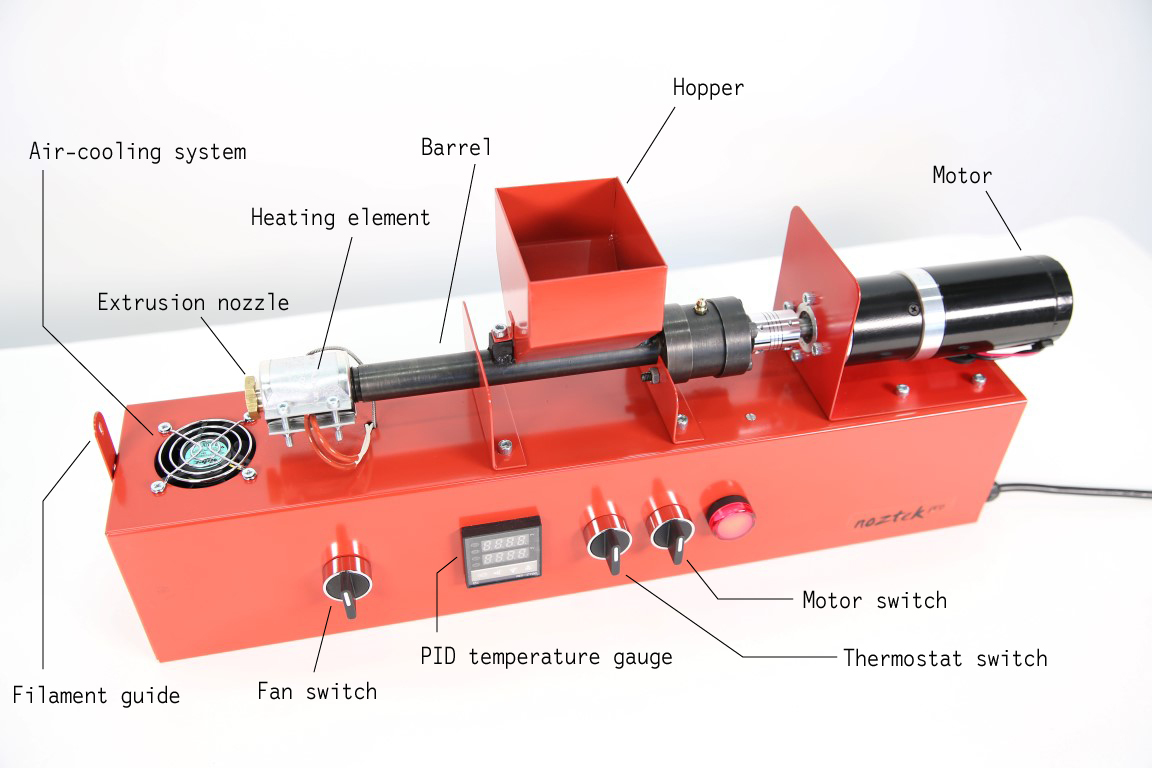
\includegraphics[scale=0.3]{Figs3//Noztekexplained.jpg}
  \caption[Details of the extruder]{\footnotesize Details of the extruder.}
  \label{Fig:extruderexp}
\end{figure}
\begin{figure}[htbp]
  \centering
  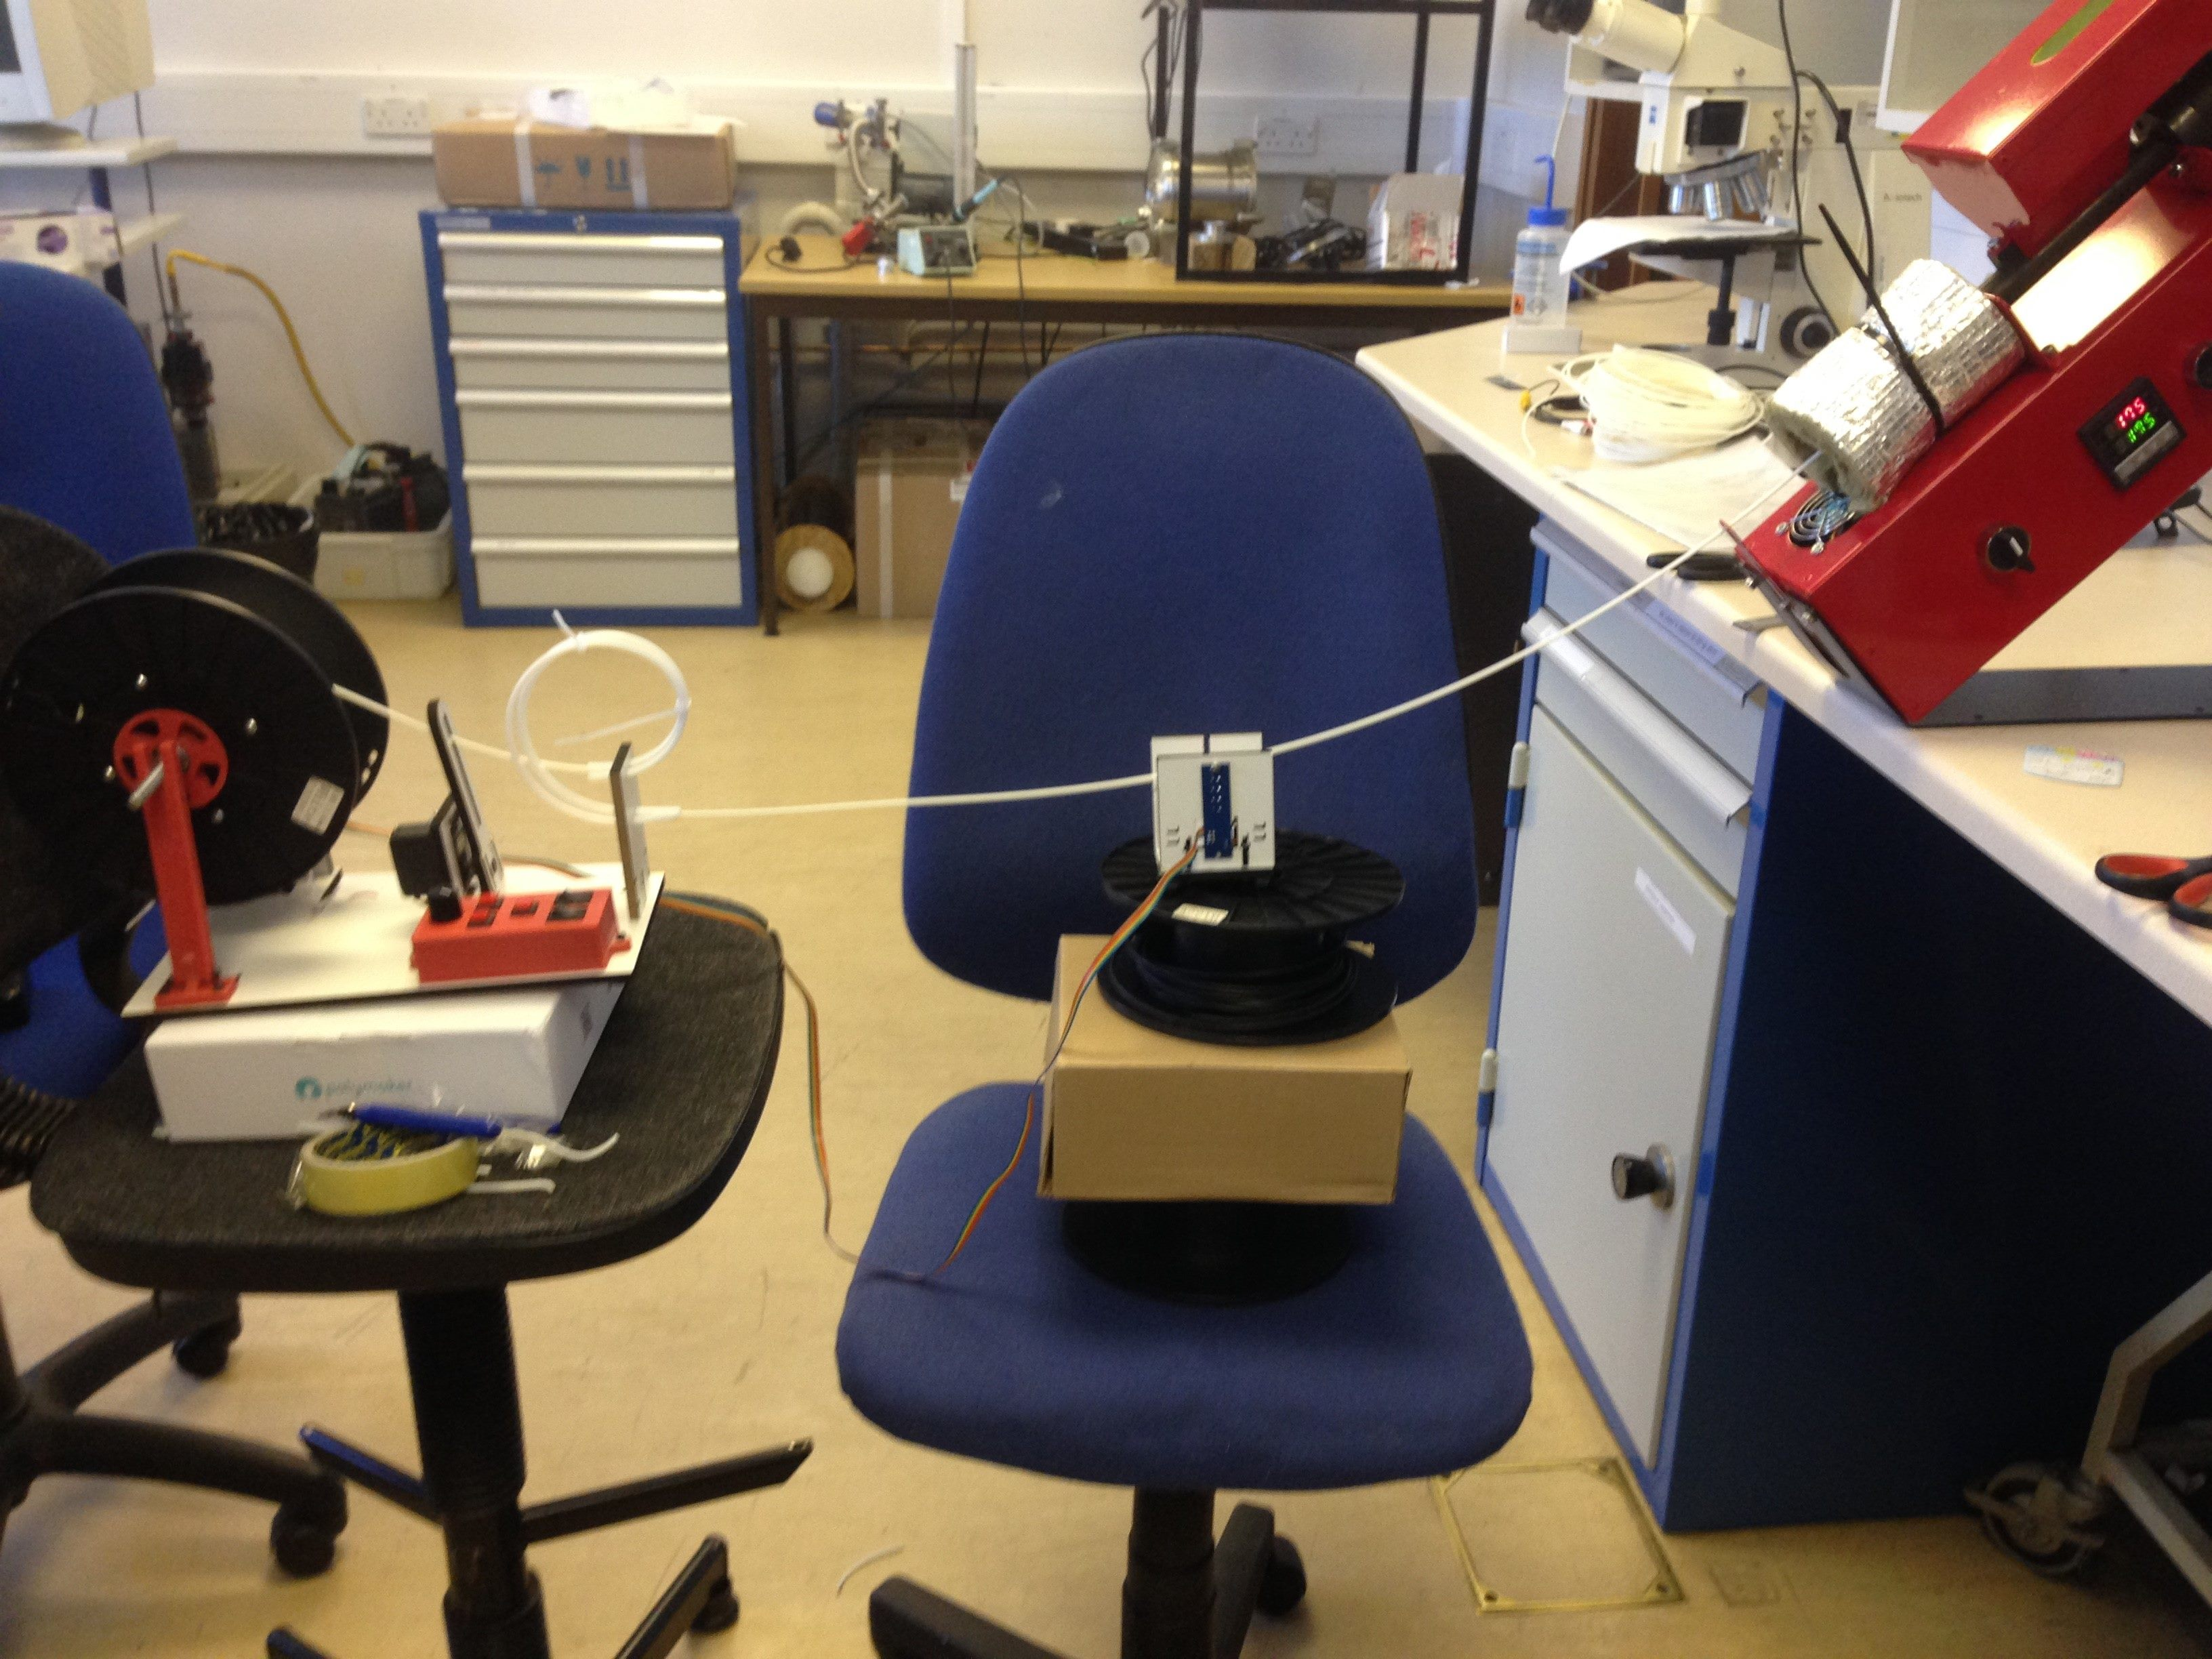
\includegraphics[scale=0.1]{Figs3//system.jpg}
  \caption[The extrusion system]{\footnotesize The extrusion system.}
  \label{Fig:system}
\end{figure}

\section{Experiment}
\subsection{Consideration of Process Parameters}
There are several settings in process we should consider in the experiment:
\begin{itemize}
\item Extruding temperature
\end{itemize}
In principle, if the extrusion speed is too slow, the temperature needs to be increased. If the filament stretches out too much or curls up right as it comes out of the nozzle, the temperature needs to be decreased. Firstly, we chose 190 $^{\circ}$C as a test according to the data sheet of the ABS pellets.
\begin{itemize}
\item Position of the sensor and winder
\end{itemize}
The location of sensor and winder depends on the whether it can control the winder’s speed appropriately which makes the filament 10-30 cm below the nozzle to avoid increased sketching. Meanwhile, it is required that the filament does not touch anything until it is cool down.
\begin{itemize}
\item Controller of the winder
\end{itemize}
The design of the filament winder offers two methods to control the winding speed:
\\
By sensor: The sensor could control the motor which is connected to the spool.It is more flexible but it needs the fine setting of the calibration and fine tuning of the position of the sensor. Since the limited sensitivity of the sensor, it might make the winder speed up sharply which causes that the filament is not uniform enough.
\\
Manually control: There is a button on the platform of the winder to control its rotating speed. This method needs more attention paid on extruder and filament. And it seems difficult to find a speed of winder which exactly corresponds to the speed of filament extruding so the speed is required to be adjusted again and again.
\begin{itemize}
\item Utilisation of fans
\end{itemize}
Since there is no water bath installation in our system, the cooling of filament depends on the air temperature and the use of fans. The air temperature in our laboratory was controlled at 24 $^{\circ}$C all the time. There are two fans we can choose. One was the small fan installed in the extruder and the other was a big fan.
Turning on the both fan would cause that the extruding temperature is not static and the diameter of the filament shrinks. But the filament could cool down faster.

\subsection{Investigation of Process Parameters}
Firstly, we compared the manual control and sensor control filament extrusion. The differences between them are not very clear. After fine calibration, the sensor could make life easier. We used sensor to control the rotation of spool in the following experiment.\\
\\
The second parameter that paid attention to was the use of fans. There was no cooling installation in our system. Only the air-conditioner in the laboratory could make progress on rapidly cooling of ABS filament. Since we want to obtain 2.85mm diameter of the filament with a 1.75mm die, it is better to cool the filament rapidly when it expands through the nozzle head.
The fan of extruder was exactly installed at the right place that the filament was very hot. Another facility that made sense was the big fan which can enable the filament to cool down entirely before it was collect by the spool.\\
\\
In the view of the idea above, we did several tests with the same position of sensor and filament winder. The diameter of the extruded filament was measured by a digital calliper at the different place of the filament. The results and corresponded parameters are described in Table \ref{tab:fan}. During the experiment, the big fan was set to the lowest power and located 50cm far from the filament to ensure the filament does not swing by the wind. The diameter of the filament is continuously variable so the measurement result is described as a range. Setting the same extruding temperature, the utilisation of any fans was detrimental to the stability of diameter. In detail, turning on the extruder fan made the filament shrinks a lot while the big fan increases the uncertainty of the diameter (changeable in a bigger range). In order to achieve a more consistent diameter and minimize the difference, it is reasonable to turn off all the fans.\\
\\
There is an interesting parameter in Table \ref{tab:fan} we should analyse as well. The extruding temperature has a strong effect on filament diameter. It was indicated that the higher extruding temperature offers a bigger filament size to some degree from 175$^{\circ}$C to 200$^{\circ}$C. This conclusion should be verified definitely by more professional work. Another principle that the higher temperature offers the faster extrusion was totally true at this stage. The most important thing was to decide an extruding temperature offering the stability and suitable size of the filament. 
\begin{table}[t]
\centering
\caption{Usages of fans for filament production}
\begin{tabular}{c c c c}
\hline
\textbf{Temperature} & \textbf{Extruder Fan} & \textbf{Big Fan} & \textbf{Filament Diameter}\\
\hline
170$^{\circ}$C & off & off & 2.65-2.75mm \\
170$^{\circ}$C & on & off & 2.60-2.72mm\\
170$^{\circ}$C & on & on & 2.41-2.61mm  \\
175$^{\circ}$C & off & off & 2.72-2.98mm \\
175$^{\circ}$C & off & on & 2.67-3.17mm\\
185$^{\circ}$C & off & off & 2.71-2.90mm \\
185$^{\circ}$C & off & on & 2.32-2.61mm\\
185$^{\circ}$C & on & off & 2.34-2.54mm  \\
190$^{\circ}$C & off & off & 2.67-2.87mm \\
190$^{\circ}$C & off & on & 2.43-2.88mm \\
190$^{\circ}$C & on & on &  2.35-2.62mm\\
200$^{\circ}$C & on & off & 2.32-2.52mm \\
200$^{\circ}$C & off & on & 2.59-2.89mm \\
200$^{\circ}$C & on & on & 2.18-2.61mm \\
\hline
\end{tabular}
\label{tab:fan}
\end{table}\\
It is time to judge the best installed position of sensor and filament winder.  
\begin{enumerate}
\item Vertical drop\\
The vertical distance is between nozzle head of extruder and the platform of filament winder. And the sensor is located in the lowest place of the extruding filament between the winder and extruder. It is general to keep winder and filament on the same horizontal platform which results in a parabola shape of extruded filament between them. It seems to require a long horizontal distance for filament flowing. In the aspect of the shrink of the filament in this way, we chose a small but non-negligible vertical drop to fabricate big size filament.
\item Horizontal distance\\
The horizontal distance means the distance between nozzle head of extruder and the guiding pipe of winder system. The setting of this parameter is related to the vertical drop, the goal is to control the stretch strength of winder to manufacture the filament with a suitable size.
\end{enumerate}
\begin{table}[t]
\centering
\caption{Extrusion parameters for filament production}
\begin{tabular}{c c c c}
\hline
\textbf{Temperature} & \textbf{Vertical Drop} & \textbf{Horizontal Distance} & \textbf{Filament Diameter}\\
\hline
170$^{\circ}$C & 30cm & 60cm & 2.65-2.75mm \\
175$^{\circ}$C & 30cm & 60cm & 2.72-2.98mm \\
175$^{\circ}$C & 25cm & 60cm & 2.87-3.03mm \\
180$^{\circ}$C & 30cm & 60cm & 2.52-2.80mm \\
180$^{\circ}$C & 30cm & 45cm & 2.95-3.04mm \\
185$^{\circ}$C & 10cm & 80cm & 2.71-2.90mm \\
190$^{\circ}$C & 10cm & 60cm & 2.67-2.87mm \\
190$^{\circ}$C & 20cm & 40cm & 2.78-3.00mm \\
195$^{\circ}$C & 20cm & 45cm & 2.72-2.89mm \\
200$^{\circ}$C & 10cm & 60cm & 2.59-2.89mm \\
200$^{\circ}$C & 20cm & 60cm & 2.64-2.84mm \\
210$^{\circ}$C & 30cm & 60cm & 2.50-2.70mm \\
220$^{\circ}$C & 20cm & 60cm & 2.45-2.65mm \\
\hline
\end{tabular}
\label{tab:tems}
\end{table}
In Table \ref{tab:tems}, there are three parameters that the size of filament contributes to. The vertical drop is related to the stability and the size of the filament. The big vertical drop increases the consistency of filament while it decreases its size. The relation between horizontal distance and diameter is obviously proportional. By analysis of these results, it is suitable to choose 20cm vertical drop and 60cm horizontal distance.  As for temperature, the range from 185$^{\circ}$C to 195$^{\circ}$C could be taken into practice.\\
\\
During the experiment, the colour of filament also attracted my attention. As can be seen in Figure \ref{Fig:filament}, the colour of filament is not uniform sometimes. Some part of it is off-white while other is white. The reason is complicated since the fabricated filament could be different even with the same settings. Our extruder is not professional and stable. But there is a need to keep the machines and ABS pellets under the good condition to improve the quality of production. 

\begin{figure}[t] % make the image in the middle of paragraph
	\centering
	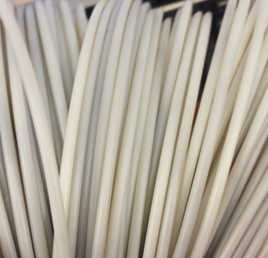
\includegraphics[scale=1]{Figs3//filament_colour.png}
  \caption[Pure ABS filament]{\footnotesize Pure ABS filament.}
  \label{Fig:filament}
\end{figure}

\section{Analysis}

According to all these results above, the optimization of all parameters could be found. It is concluded that there is a high probability to manufacture 2.85mm filament with 195$^{\circ}$C extruding temperature, 20cm vertical drop and 60cm horizontal distance. The best result with these settings is the filament at 2.85 $\pm$ 0.07mm. The diameter error is controlled within 2.5\%.\\ 
\\
It can not be avoided that the diameter of the filament is changeable because the extruding speed and filament wind speed are not stable. The extruder we used is not professional and the extruding system is simplified which may cause some weakness. Actually, the filament we bought does not have a specific diameter (e.g. 3.00 $\pm$ 0.05mm). This diameter tolerance (i.e. 0.05 mm) the gold standard across the industry. In this case, the filament we produced seems to been printable in Ultimaker 2 printer in the aspect of its diameter.\\
\\
As for the colour of filament, it does not make a big difference to its printing properties. Since the screw in the extruder is not long enough, the extrusion process is simplified. There is an uncertainty of the production because of the insufficient extruding.The tip is keeping the nozzle at the extruding temperature at least 20 minutes before the extrusion starts. And it is necessary to check the connection of every part and clean the hopper.\\
\\
It is also significant to storage our filament in an air tight container in order to print high-quality products\cite{abs}. The tricky thing with most thermoplastics is the moisture absorption, which results in small water bubbles in the filament. It will bring pops when extruding it in 3D printer. The extruding temperature is usually higher than the boiling point of water so that the water explodes violently. Obviously,  the quality of our 3D prints dramatically destroys since the material is spewed out randomly, instead of being correctly laid down. Also, it could cause spluttering and problems with adhesion on the base layer of the prints. There is a basic strategy to keep your 3D printing filament and avoid the accumulation of water from the atmosphere. It is very effective to store the filament in an air tight desiccator with a small silica gel desiccant pouch.\\
